\RequirePackage[T1]{fontenc}
\documentclass[conference,letterpaper]{IEEEtran}
\usepackage{amsmath,amssymb,booktabs,array,graphicx}
\usepackage{balance}
\usepackage{tikz}
\usetikzlibrary{arrows.meta,positioning}
\usepackage[hidelinks]{hyperref}
\title{CHIA-MACO-FMCW: Reproducible Compiler--Architecture Exploration for a Radar Pipeline}
\author{\IEEEauthorblockN{Zesong Jiang, Cheng Tan, Jeff Zhang}
\IEEEauthorblockA{Arizona State University}}
\begin{document}
\maketitle
\begin{abstract}
We present a CHIA workflow for compiler--architecture exploration of a frequency-modulated continuous-wave (FMCW) radar pipeline on a coarse-grained reconfigurable array (CGRA). Four original MACO agent roles, driven by Qwen3.8-27B, propose and rank bounded array/unroll configurations and learn from real mapper feedback. In one three-round run, 12 model calls and 18 unique mappings find the same 39.15-million-cycle estimate as a 36-mapping exhaustive reference, but require more wall time. The reference identifies $2\times2$ and $4\times4$ arrays on the cycle/tile frontier; $4\times4$ is 4.86\% below its scalar estimate, while a larger $6\times6$ array is worse. The artifact includes an executable C workload, model traces, mapper logs and a live GUI. Results use an analytical model built from mapper initiation intervals, not cycle-accurate simulation or physical-design measurements.
\end{abstract}

\section{Introduction}
FMCW radar processing combines stages with different computational structures. Windowing performs regular elementwise arithmetic, FFTs perform complex butterflies, transposition changes data layout, power accumulation reduces across receivers, and two-dimensional cell-averaging constant-false-alarm-rate (CA-CFAR) detection aggregates neighborhoods of a range--Doppler map. Range--Doppler detection motivates joint consideration of these stages~\cite{cfar}. A compiler setting that benefits one kernel may offer little benefit for the complete frame.

CGRA co-design couples the program representation and its mapping to the processing array. MACO studies this coupling through a multi-agent design workflow~\cite{maco}. This hackathon artifact isolates a smaller, reproducible question: what compiler/array tradeoffs can a CHIA workflow expose for one radar workload using a real LLVM-based mapper? CHIA supplies a composable execution interface for hardware/software research workflows~\cite{chia}; CGRA-Mapper supplies loop extraction and mapping for parameterized arrays~\cite{opencgra}.

Our contributions are an executable FMCW C workload, mapping views with explicit loop selection, a MACO-agent/CHIA feedback loop, and a deterministic 36-evaluation reference search. Both policies use the same evaluator and frame-cost model. The agent experiment is a bounded adaptation, not a reproduction of MACO's full PPA optimization.

\section{Workload and CHIA Workflow}
\subsection{Executable workload}
The nominal input contains 256 samples per chirp, 128 chirps per frame, and four receive channels. The native reference uses single-precision complex values and executes Hann windowing, radix-2 range FFTs, transposition, Doppler FFTs, power accumulation, and CA-CFAR. Beamforming and tracking are outside its scope.

A native smoke test injects a noiseless target at range bin 17 and Doppler bin 9. The compiled program recovers that peak and emits a power checksum of approximately $1.60432109\times10^9$. This is a functional test of the reference pipeline. The scene does not establish detection probability, false-alarm performance, or robustness to noise. In particular, a recovered peak should not be interpreted as validation of every CFAR detection in a noiseless scene.

A subsequent independent NumPy comparison covers six deterministic scenes. Range FFT, Doppler FFT and power outputs all satisfy a predefined normalized maximum-error bound of $2\times10^{-5}$. However, exact full-mask CFAR equality passes only the noisy-target and zero-input scenes. The four noiseless scenes differ at near-zero-power bins; the single-target case has 1,343 differing decisions. These failures are retained rather than relaxing the pass criterion. This validates neither mapped kernels nor candidate hardware.

\subsection{Candidate and evaluator contracts}
A candidate specifies the kernel, array dimensions, source unroll factor, and fixed mapping parameters. The evaluator compiles a mapping view with LLVM 12, extracts its dataflow graph (DFG), and invokes CGRA-Mapper in a Docker container. Parsed results include mapping success, initiation interval (II), resource and recurrence lower bounds, DFG node/edge counts, and reported functional-unit and crossbar utilization.

\begin{figure}[t]
\centering
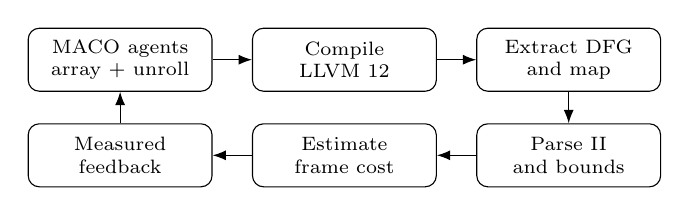
\begin{tikzpicture}[node distance=4mm and 5mm,>=Latex,
 box/.style={draw,rounded corners,align=center,font=\scriptsize,
 text width=21mm,minimum height=8mm}]
\node[box] (enum) {MACO agents\\array + unroll};
\node[box,right=of enum] (compile) {Compile\\LLVM 12};
\node[box,right=of compile] (map) {Extract DFG\\and map};
\node[box,below=of map] (parse) {Parse II\\and bounds};
\node[box,left=of parse] (model) {Estimate\\frame cost};
\node[box,left=of model] (archive) {Measured\\feedback};
\draw[->] (enum)--(compile);
\draw[->] (compile)--(map);
\draw[->] (map)--(parse);
\draw[->] (parse)--(model);
\draw[->] (model)--(archive);
\draw[->] (archive)--(enum);
\end{tikzpicture}
\caption{Agent loop. Four MACO roles propose, repair, screen and predict; CHIA executes real mappings before measurements feed the next round. Enumeration replaces the agent policy for the reference search.}
\label{fig:loop}
\end{figure}

Figure~\ref{fig:loop} summarizes the workflow. CHIA schedules the evaluator through a declared mapper resource. Each invocation has a unique container name and a 60-second timeout. A failed or timed-out evaluation returns a structured failure rather than a favorable cost. These interfaces allow the outer search policy to change without changing the tool or result contract.

\subsection{MACO agent policy}
The original MACO Co-designer, Fixer, Coarse Judge and Fine Judge classes share a local Qwen3.8-27B raw model, served with NF4 double quantization. An adapter supplies the transport and bounded schema; no HARP-trained policy is used. Each of three rounds proposes two full-frame plans, repairs invalid settings, ranks the shortlist and predicts a winner. Every shortlisted plan that fits the 30-mapping budget is measured through CHIA. Only this run's measurements are cached and fed back; the exhaustive archive is never provided to the model.

Exploration hints follow a decaying-epsilon schedule. Prediction confidence is updated from measured cycle regret but never substitutes for tool validation. This deliberately omits MACO's confidence-based tool skipping and synthesis/PPA evaluator. Model output is limited to 384 tokens per call; malformed output fails visibly rather than triggering a random fallback. Full prompts, responses, usage, source hashes and mapper logs are retained.

\subsection{Correct loop selection}
CGRA-Mapper targets a selected loop in the LLVM representation. An early runtime-unroll experiment appeared favorable, but log inspection showed that the mapper selected a scalar cleanup loop instead of the intended unrolled body. Those results were excluded from the reported search.

The final \texttt{fmcw\_mapping.c} exposes one fixed-shape top-level loop per stage, with explicit source-level unrolling. This makes the mapping target unambiguous. The complete native implementation remains the functional reference. A mapper success establishes schedulability of the extracted DFG; it does not by itself prove numerical equivalence between a mapping view and every dynamic invocation in the native program.

DFG statistics support the audit: the selected $4\times4$ window view has 59 nodes at unroll four, versus 17 in its scalar view. Node count helps detect suspicious extraction but is not a semantic proof.

\section{Search Space and Cost Model}
\subsection{Bounded compiler--array search}
We evaluate $2\times2$, $4\times4$, and $6\times6$ square arrays under the same mapper template. Legal unroll factors are $\{1,2,4\}$ for windowing, transpose, and power; $\{1,2\}$ for FFT; and $\{1\}$ for CFAR. The resulting space contains 12 kernel configurations per array and 36 mapper evaluations.

CFAR unrolling is excluded from the final bounded space after exploratory larger-DFG evaluations exceeded the time budget. Thus, the reported mapping success rate applies to the retained legal space. Architecture exploration varies array dimensions; it does not vary functional-unit mix, memory banking, or interconnect topology.

For each array, we select the lowest estimated cost among successful compiler settings for each kernel. Because the model sums independent kernel costs, these selections can be made separately without enumerating every combination of stage settings. Cross-stage fusion, shared-memory constraints, or overlapping execution would invalidate that separability and require a different search formulation.

\subsection{Counting scheduled work}
Let $\mathcal I_k$ be the dynamic invocations of the mapped loop for stage $k$, and let $n_{k,j}$ denote its iteration count in invocation $j$. With unroll factor $u_k$, the model is
\begin{align}
G_k(u_k)&=\sum_{j\in\mathcal I_k}
             \left\lceil n_{k,j}/u_k\right\rceil,\\
\widehat C_{\mathrm{frame}}&=\sum_k G_k(u_k)\,\mathrm{II}_k.
\end{align}
Rounding occurs per invocation, not once after summing iterations. This matters for the short inner loops of early FFT stages. For example, the FFT has 983,040 scalar butterflies per frame, but unroll two yields 557,056 scheduled groups in the artifact's accounting, rather than simply half the scalar count.

\begin{table}[t]
\caption{Scalar work counted by the frame model}
\label{tab:work}
\centering\small
\begin{tabular}{lr}
\toprule
Mapped operation & Iterations/frame\\
\midrule
Window sample & 131,072\\
FFT butterfly (range + Doppler) & 983,040\\
Transpose copy (two passes) & 262,144\\
Receiver power accumulation & 131,072\\
CFAR neighborhood-loop visit & 3,512,388\\
\bottomrule
\end{tabular}
\end{table}

Table~\ref{tab:work} lists the scalar counts. The transpose term includes two passes. The CFAR term counts $(256-10)(128-10)11^2$ neighborhood-loop visits for interior cells with outer radius five. It is not the number of detected targets or the number of output pixels.

The estimate excludes loop setup, FFT bit reversal, memory stalls, host/CGRA transfers, and pipeline fill/drain. It also applies one measured stage II across the modeled invocations. The use of short FFT loops makes this an approximation even after invocation-level rounding. Tile count is a size proxy, not synthesized area. No clock frequency is measured, so estimated cycles are not converted into throughput or energy.

\section{Results and Findings}
The archived CHIA run completed all 36 mappings successfully in 38.71 seconds. Table~\ref{tab:results} compares the selected compiler settings with the scalar setting on the same array. Percentages describe reductions in the analytical estimate, not measured application speedups.

\subsection{Agent-guided run}
The GUI-launched seed-37 run completed three rounds, 12 model calls and 18 successful unique mappings in 210.43 seconds, with 29,657 prompt and 1,700 completion tokens. Its measured best improved from 40,170,152 cycles in round one to 39,154,344 in round three, using $4\times4$ and unroll factors $[4,2,4,4,1]$. This is an actually proposed and evaluated full-frame plan, not a combination assembled after search. Round two repeated existing plans; the within-run cache avoided redundant mappings.

The agent matched the exhaustive reference's best estimate with half as many unique mappings, but was slower overall because of model-call overhead. These are descriptive results from one seed, not a matched-budget efficiency claim. An earlier integration trial stopped on truncated judge JSON at the service's 384-token limit; a stricter rationale-length contract resolved this in the reported run. The failed trace is retained, not converted into a successful result.

\begin{table}[t]
\caption{Array comparison: estimated millions of cycles/frame}
\label{tab:results}
\centering\small
\begin{tabular}{lrrrr}
\toprule
Array & Tiles & Scalar & Selected & Reduction\\
\midrule
$2\times2$ & 4 & 46.199 & 45.479 & 1.56\%\\
$4\times4$ & 16 & 41.153 & 39.154 & 4.86\%\\
$6\times6$ & 36 & 44.666 & 41.946 & 6.09\%\\
\bottomrule
\end{tabular}
\end{table}

\subsection{Array size is not monotonic}
The $4\times4$ array has the lowest estimate, 39,154,344 cycles. The $6\times6$ array has a 7.13\% higher estimate despite using $2.25\times$ as many tiles. Its scalar CFAR II is 11, compared with 10 for both smaller arrays. Since CFAR dominates total modeled work, this one-cycle change outweighs improvements in the other stages.

This observation concerns a heuristic mapper and a fixed architecture template. It does not prove that the larger array is intrinsically inferior or that no better mapping exists. Instead, it demonstrates why tool feedback is needed: greater nominal compute capacity did not translate into a better schedule for the dominant loop in this run.

\begin{figure}[t]
\centering
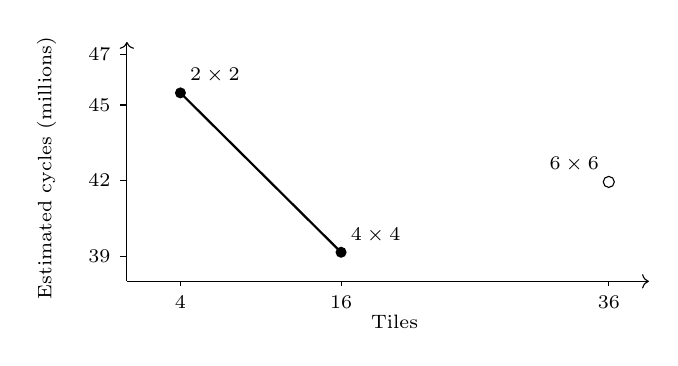
\begin{tikzpicture}[x=0.17cm,y=0.32cm,font=\scriptsize]
\draw[->] (0,38)--(39,38);
\node at (20,36.4) {Tiles};
\draw[->] (0,38)--(0,47.5);
\foreach \x in {4,16,36}
 {\draw (\x,38)--(\x,37.8) node[below]{\x};}
\foreach \y in {39,42,45,47}
 {\draw (0,\y)--(-0.5,\y) node[left]{\y};}
\node[rotate=90] at (-6,42.5) {Estimated cycles (millions)};
\draw[thick] (4,45.478568)--(16,39.154344);
\fill (4,45.478568) circle(2pt) node[above right]{$2\times2$};
\fill (16,39.154344) circle(2pt) node[above right]{$4\times4$};
\draw[fill=white] (36,41.945836) circle(2pt) node[above left]{$6\times6$};
\end{tikzpicture}
\caption{Cycle/tile frontier from the archived run. Filled points are nondominated; $6\times6$ is dominated by $4\times4$.}
\label{fig:pareto}
\end{figure}

\subsection{Compiler choice and the dominant stage}
Table~\ref{tab:compiler} gives the selected $4\times4$ settings. Unrolling increases DFG size and can increase raw II, but can still reduce estimated cost because each scheduled group covers more work. Accordingly, the selector minimizes $G_k\mathrm{II}_k$, not II alone.

\begin{table}[t]
\caption{Selected compiler settings for the $4\times4$ array}
\label{tab:compiler}
\centering\small
\begin{tabular}{lrrr}
\toprule
Stage & Unroll & II & DFG nodes\\
\midrule
Window & 4 & 7 & 59\\
FFT & 2 & 6 & 59\\
Transpose & 4 & 5 & 35\\
Power & 4 & 4 & 44\\
CA-CFAR & 1 & 10 & 20\\
\bottomrule
\end{tabular}
\end{table}

CFAR contributes 35,123,880 cycles, or 89.7\% of the selected $4\times4$ total. Improvements to windowing or power accumulation alone therefore have limited effect on the frame estimate. This finding directs subsequent work toward the neighborhood reduction and its data reuse. A faster CFAR formulation would need both a correctness check and a revised cost model; an assumed reduction cannot be inserted into the measured result.

Figure~\ref{fig:pareto} shows two useful choices. The $2\times2$ array minimizes the cycle--tile product, while $4\times4$ minimizes estimated latency. Reporting both avoids treating a proxy-weighted objective as a universal best design. A physical-area budget or memory constraint could change the preferred point.

\section{Artifact and Reproduction}
The \texttt{chia-maco} directory contains the workload, mapping views, evaluator, CHIA node, search code, tests and result JSON. The exhaustive reference is \path{results/codesign_search_certified.json}; the reported agent run is \path{results/agent_qwen38_27b_seed37_v3/}. These retain the measurements, selected settings and provenance used in this paper.

The tested setup uses Python 3.10, CHIA 1.0.1 at commit \texttt{16c35e9}, and LLVM 12 inside \texttt{cgramapper:v1}. In \texttt{chia-maco}, \texttt{make smoke}, \texttt{make test}, and \texttt{make codesign-search} check the C workload, contracts, and exhaustive reference. The \texttt{agent-search} CLI runs the agent loop with a new output directory; the README documents model endpoint configuration. The independent MACO browser GUI launches the same loop and displays role progress, model usage, decisions, measured winners and failures. Automated checks cover agent contracts, caching, budgets, feedback and project-isolated APIs.

The reference archive contains parsed records; the agent archive additionally includes raw mapper logs and model traces. Reused MACO modules are pinned to commit \texttt{31c02ce}. Redistribution licenses and the public release URL must be confirmed before submission.

\section{Limitations and Next Steps}
The original proposal targeted 16-bit inputs, simulation, synthesis-calibrated PPA, and at least 20 frames/s. The current experiment uses floating-point C, six software-validation scenes, heuristic mapping, and a steady-state estimate. It does not establish fixed-point accuracy or those system-level targets.

An export audit found lost floating-point opcodes, misclassified squares, and a comparison-predicate mismatch. We recover these from LLVM evidence and correct the wrapper's HardFloat format parameters. Translated Verilog tests pass 1,568 bit-exact FP32 results and nine unsigned comparisons at both FU and isolated-tile levels, including control loading and backpressure. These programs do not execute the mapper schedule. Operand translation, constant/address loading, and whole-frame execution remain unfinished. Component tests therefore do not certify candidate hardware correctness.

The search contains three arrays and restricted unrolling. A single-seed agent demonstration does not establish search efficiency; no matched-budget evolutionary comparison is reported. Kernel mappings are not independently validated end-to-end accelerators. Mapping views and analytical aggregation omit the hardware interface between stages.

Next steps are resolving the CFAR numerical discrepancies, compiler-to-RTL integration, explicit-memory simulation and synthesis. Hardware performance claims require those checks; multi-seed, matched-budget studies are also needed to assess the agent policy.

\balance
\section{Conclusion}
CHIA-MACO-FMCW connects original MACO agents to real CHIA compiler/mapper feedback. One bounded Qwen run matched the exhaustive best with fewer mappings but higher elapsed time. The reference identifies two Pareto choices and CFAR as the dominant modeled cost. The reusable contribution is an inspectable agent/tool loop with explicit contracts, failures and model limitations.

\begin{thebibliography}{4}
\bibitem{cfar} M. Kronauge and H. Rohling, \emph{Fast two-dimensional CFAR procedure}, IEEE Trans. Aerospace and Electronic Systems, vol. 49, no. 3, pp. 1817--1823, 2013.
\bibitem{maco} Z. Jiang et al., \emph{MACO: A multi-agent LLM framework for automated CGRA hardware/software co-design}, arXiv:2509.13557, 2025, revised 2026.
\bibitem{chia} A. Cui et al., \emph{CHIA: An open-source framework for principled, agentic AI-driven hardware/software co-design research}, arXiv:2606.27350, 2026.
\bibitem{opencgra} C. Tan, C. Xie, A. Li, K. J. Barker, and A. Tumeo, \emph{OpenCGRA: An open-source unified framework for modeling, testing, and evaluating CGRAs}, ICCD, 2020, pp. 381--388.
\end{thebibliography}
\section*{Acknowledgment of AI Assistance}
OpenAI Codex assisted with drafting, editing, and LaTeX preparation of this paper, as well as artifact implementation and experiment scripting. The human authors are responsible for the entire contents, tone, and quality of the paper, including its claims and reported results.
\end{document}
